%!TEX root = practicum2.tex
\todo[inline]{Hoe verandert de fractal dimension $\rho$ als een functie van $p$?}

\textcite{falconer2004fractal} describes the fractal dimension as some number $\rho$ such that
\begin{equation}
	M_\varepsilon(\rho) \sim c\varepsilon^{-s}
\end{equation}
where $c$ and $s$ are constants and $M_\varepsilon(\rho)$ are measurements at different scales $\varepsilon$ for $\varepsilon \to 0$. \citeauthor{falconer2004fractal} then shows that the fractal dimension can be estimated ``as minus the gradient of a log-log graph plotted over a suitable range of $\varepsilon$"\cite{falconer2004fractal}. 
\todo[inline]{Wat is delta?}

	% \begin{equation}
	% 	\text{dim}_{\text{box}} = \lim_{\epsilon \to 0} \frac{\log N(\epsilon)}{\log\left[ \frac{1}{\epsilon} \right]}.
	% \end{equation}
One way to get the measurements $M_\varepsilon$ is to use box-counting. When box-counting is used the different scales mentioned in \citeauthor{falconer2004fractal}'s definition are the sizes of the boxes. \todo[inline]{Boxcounting uitleggen}

We have used the function \t{box-count} by \textcite{boxCounting} to determine the fractal dimension of Percolation clusters. This method uses box sizes that are power of two. Consequently $\varepsilon = 1, 2, 4, \dotsc 2^q$ where $q$ is the smallest integer such that $q \leq (2N + 1)$. 

We have used the box-counting algorithm on a cluster generated with $N = 80$, $p = 0.7$, the used cluster is shown in \cref{fig:exp_fractal:cluster}. \Cref{fig:exp_fractal:fractalDimension} presents the number of boxes as a function of the size of the boxes. \todo[inline]{Uileggen hoe we dimension uit dit figuur halen.} The box-counting dimension can be read from \cref{fig:exp_fractal:fractalDimensionGradient} to be \num{1.879}, which neatly approximates the dimension \num{1.896} mentioned by \textcite{stauffer1994introduction}. The small difference between these numbers can be explained by the relatively small size of our cluster. 

\begin{figure*}
	\centering
	\begin{subfigure}[t]{0.3\textwidth}
		\centering
		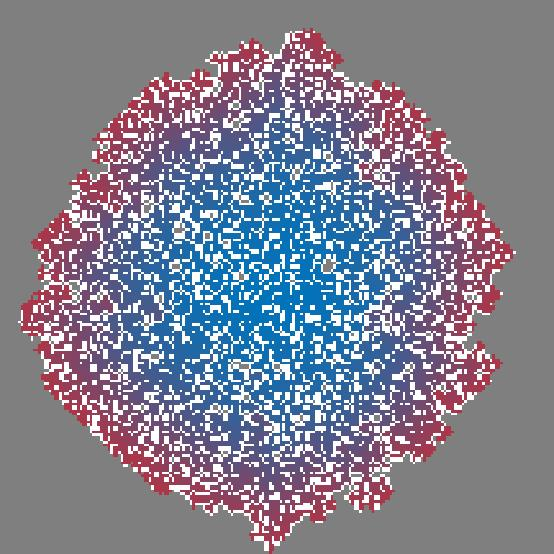
\includegraphics[width=1\textwidth]{./img/assignment_fractal_cluster}
		\caption{The cluster.}
		\label{fig:exp_fractal:cluster}
	\end{subfigure}
	\begin{subfigure}[t]{0.3\textwidth}
		\centering
		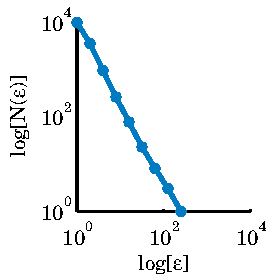
\includegraphics[width=1\textwidth]{./img/assignment_fractal_numboxesVSboxsize}
		\caption{The number of boxes as function of the box size.}
		\label{fig:exp_fractal:fractalDimension}	
	\end{subfigure}	
	\begin{subfigure}[t]{0.3\textwidth}
		\centering
		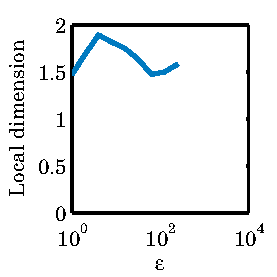
\includegraphics[width=1\textwidth]{./img/assignment_fractal_gradient}
		\caption{The gradient of \cref{fig:exp_fractal:fractalDimension}.}
		\label{fig:exp_fractal:fractalDimensionGradient}
	\end{subfigure}		
	\caption{\subref{fig:exp_fractal:cluster} The cluster ($N = 80, p = 0.7$) used to compute the box-counting dimension. \subref{fig:exp_fractal:fractalDimension} The number of boxes used to cover that cluster as a function of the box size. \subref{fig:exp_fractal:fractalDimensionGradient} The gradient of the function plotted in \subref{fig:exp_fractal:fractalDimension}.}
	\label{fig:exp:dimension:plaatjes}
\end{figure*}

